\documentclass{article}

\usepackage{arxiv}

\usepackage[utf8]{inputenc} % allow utf-8 input
\usepackage[T1]{fontenc}    % use 8-bit T1 fonts
\usepackage{hyperref}       % hyperlinks
\usepackage{url}            % simple URL typesetting
\usepackage{booktabs}       % professional-quality tables
\usepackage{amsfonts}       % blackboard math symbols
\usepackage{nicefrac}       % compact symbols for 1/2, etc.
\usepackage{microtype}      % microtypography

\usepackage{graphicx}

\usepackage{lipsum}		% Can be removed after putting your text content

\newtheorem{definition}{Definition}
\newtheorem{lemma}{Lemma}
\newtheorem{proposition}{Proposition}
\newtheorem{program}{Program}
\newtheorem{convention}{Convention}

\title{Notes on geometrical interpretation of adjoint equation}

%\date{September 9, 1985}	% Here you can change the date presented in the paper title
%\date{} 					% Or removing it

\author{
  Mingli~Yuan \\
  AI Lab \\
  Beijing ColorfulClouds Tech.\\
  Beijing, 100083 \\
  \texttt{mingli.yuan@caiyunapp.com} \\
  %% examples of more authors
  %% \AND
  %% Coauthor \\
  %% Affiliation \\
  %% Address \\
  %% \texttt{email} \\
  %% \And
  %% Coauthor \\
  %% Affiliation \\
  %% Address \\
  %% \texttt{email} \\
  %% \And
  %% Coauthor \\
  %% Affiliation \\
  %% Address \\
  %% \texttt{email} \\
}

% Uncomment to remove the date
%\date{}

% Uncomment to override  the `A preprint' in the header
%\renewcommand{\headeright}{Technical Report}
%\renewcommand{\undertitle}{Technical Report}

\begin{document}
\maketitle

\begin{abstract}
Traditionally, adjoint equation was introduced via the technic of integration-by-part.
After recalling the geometrical interpretation of adjoint in linear cases,
we reveal that adjoint equation shares the same interpretation,
and then a new dual-number-based definition of adjoint equation and proof for equivalence between definitions are given.
\end{abstract}

\keywords{adjoint \and adjoint equation \and geometrical interpretation \and dual number}

\section{Introduction}

The concept of adjoint is very fundamental, and adjoint equation shows its importance in domains of optimal control, sensitivity analysis, and data assimilation. Also, recent contribution shows adjoint equation can play a role in the intersection area of deep learning and differential equations.

In linear cases, there is an apparent geometrical interpretation of adjoint, and in this paper, we want to reveal adjoint equation shares the same interpretation.

\subsection{Geometrical interpretation for adjoint in linear case}

\begin{definition}
\label{d0}
A dual system $ \langle X, Y \rangle $ is a bilinear mapping $ \langle , \rangle : X \times Y \to F $ where $X$, $Y$ are two vector space and $ F $ is a field.
\end{definition}

\begin{convention}
We call $ X $ in $ \langle X, Y \rangle $ is a bottom space, $ Y $ is a frame space, and the value of $ \langle x, y \rangle $ is a coordinate.
\end{convention}

\begin{figure}[ht]
\centering
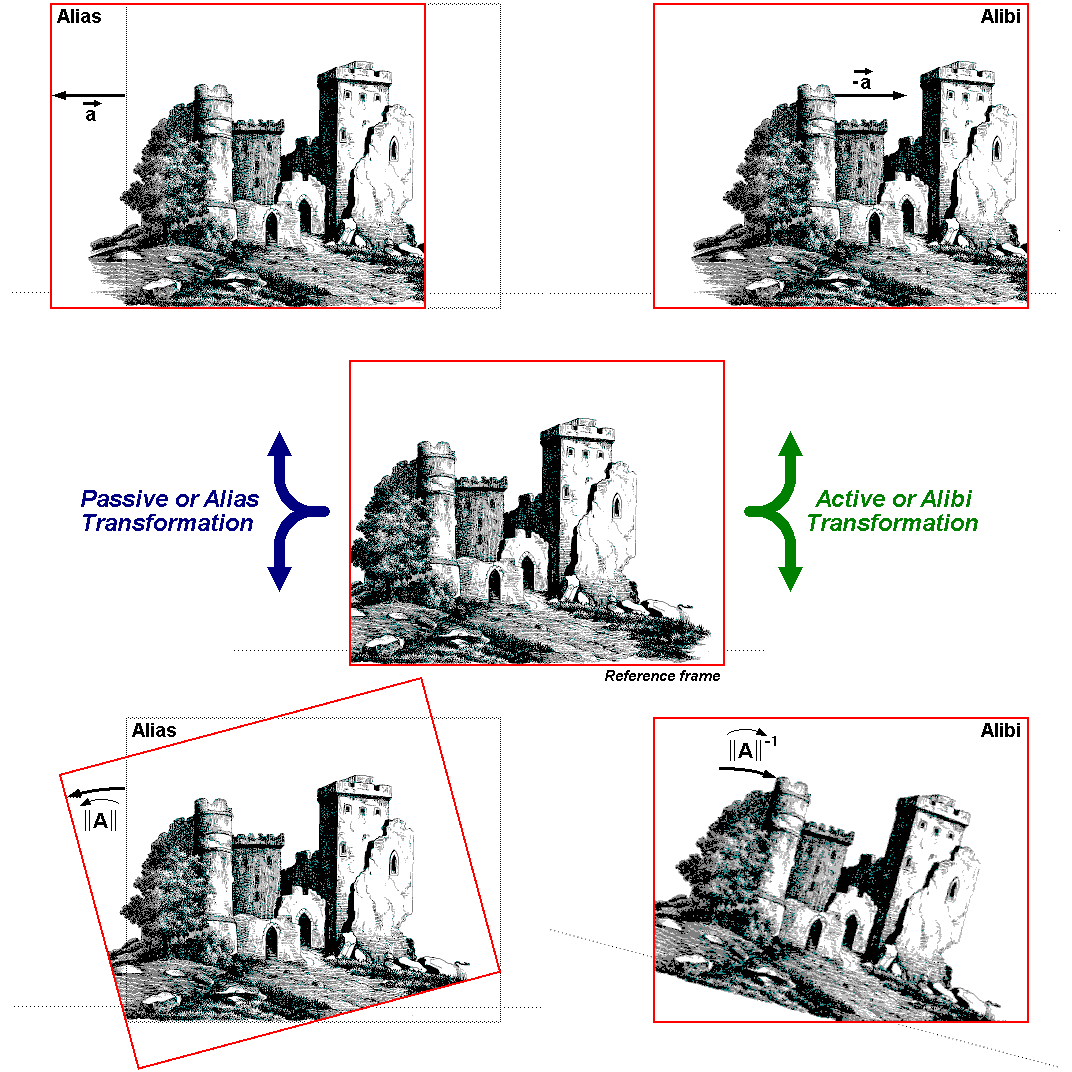
\includegraphics[width=3.5in]{../images/adjoint/alias_and_alibi.png}
\caption{A dual system and two pair of operators}
\end{figure}

\begin{definition}
\label{d1}
For two dual system $ \langle X_1, Y_1 \rangle $ and $ \langle X_2, Y_2 \rangle $ , each of the two operator $ A : X_1 \to X_2$ and $ B : Y_2 \to Y_1 $ is an adjoint of the other counterpart,
if and only if, the equation $$ \langle A \phi, \psi \rangle = \langle \phi, B \psi \rangle $$ holds for arbitrary $ \phi \in X_1 $ and $ \psi \in Y_2 $
\end{definition}

\subsection{The traditional way to introduce adjoint equation}

\subsection{Adjoint equation in deep learning}

\section{Geometrical interpretation of adjoint equation}

\subsection{Additional and multiplicational point of view}

\subsection{Forward and backward propagation of a disturbance}

\subsection{The geometrical interpretation}


\section{Reformulate with dual number}


\section{Applications}

\lipsum[8] \cite{kour2014real,kour2014fast} and see \cite{hadash2018estimate}.

The documentation for \verb+natbib+ may be found at
\begin{center}
  \url{http://mirrors.ctan.org/macros/latex/contrib/natbib/natnotes.pdf}
\end{center}
Of note is the command \verb+\citet+, which produces citations
appropriate for use in inline text.  For example,
\begin{verbatim}
   \citet{hasselmo} investigated\dots
\end{verbatim}
produces
\begin{quote}
  Hasselmo, et al.\ (1995) investigated\dots
\end{quote}

\begin{center}
  \url{https://www.ctan.org/pkg/booktabs}
\end{center}


\subsection{Figures}
\lipsum[10] 
See Figure \ref{fig:fig1}. Here is how you add footnotes. \footnote{Sample of the first footnote.}
\lipsum[11] 

\begin{figure}
  \centering
  \fbox{\rule[-.5cm]{4cm}{4cm} \rule[-.5cm]{4cm}{0cm}}
  \caption{Sample figure caption.}
  \label{fig:fig1}
\end{figure}

\subsection{Tables}
\lipsum[12]
See awesome Table~\ref{tab:table}.

\begin{table}
 \caption{Sample table title}
  \centering
  \begin{tabular}{lll}
    \toprule
    \multicolumn{2}{c}{Part}                   \\
    \cmidrule(r){1-2}
    Name     & Description     & Size ($\mu$m) \\
    \midrule
    Dendrite & Input terminal  & $\sim$100     \\
    Axon     & Output terminal & $\sim$10      \\
    Soma     & Cell body       & up to $10^6$  \\
    \bottomrule
  \end{tabular}
  \label{tab:table}
\end{table}

\subsection{Lists}
\begin{itemize}
\item Lorem ipsum dolor sit amet
\item consectetur adipiscing elit. 
\item Aliquam dignissim blandit est, in dictum tortor gravida eget. In ac rutrum magna.
\end{itemize}


\bibliographystyle{unsrt}  
%\bibliography{references}  %%% Remove comment to use the external .bib file (using bibtex).
%%% and comment out the ``thebibliography'' section.


%%% Comment out this section when you \bibliography{references} is enabled.
\begin{thebibliography}{1}

\bibitem{kour2014real}
George Kour and Raid Saabne.
\newblock Real-time segmentation of on-line handwritten arabic script.
\newblock In {\em Frontiers in Handwriting Recognition (ICFHR), 2014 14th
  International Conference on}, pages 417--422. IEEE, 2014.

\bibitem{kour2014fast}
George Kour and Raid Saabne.
\newblock Fast classification of handwritten on-line arabic characters.
\newblock In {\em Soft Computing and Pattern Recognition (SoCPaR), 2014 6th
  International Conference of}, pages 312--318. IEEE, 2014.

\bibitem{hadash2018estimate}
Guy Hadash, Einat Kermany, Boaz Carmeli, Ofer Lavi, George Kour, and Alon
  Jacovi.
\newblock Estimate and replace: A novel approach to integrating deep neural
  networks with existing applications.
\newblock {\em arXiv preprint arXiv:1804.09028}, 2018.

\end{thebibliography}


\end{document}
